\documentclass[xcolor={dvipsnames},aspectratio=169,10pt]{beamer}

% chktex-file 41

% check for obsoleted LaTeX packages
\usepackage[l2tabu,orthodox]{nag}

% utility packages
\usepackage{etoolbox}
\usepackage{xifthen}
\usepackage{xpatch}
\usepackage{adjustbox}

% better text justifying
\usepackage{microtype}
% justify text inside list environment
% Ref: http://liam0205.me/2017/04/11/justifying-in-beamer-s-lists/
\usepackage{ragged2e}
\makeatletter
\xpatchcmd{\itemize}{\raggedright}{\justifying}{}{}
\xpatchcmd{\beamer@enum@}{\raggedright}{\justifying}{}{}
\xpatchcmd{\@@description}{\raggedright}{\justifying}{}{}
\makeatother

% math related packages
\usepackage{amsmath}
\usepackage{amssymb}
\let\emptyset\varnothing%
\usepackage{amsfonts}
\usepackage{mathrsfs}
\usepackage{latexsym}
\usepackage{bm}
\usepackage{fancynum}

% equation style
\newcommand{\setdisplayskip}{%
  \abovedisplayskip=0.25\baselineskip plus 0.05\baselineskip minus 0.125\baselineskip% chktex 1
  \abovedisplayshortskip=0pt plus 0.075\baselineskip% chktex 1
  \belowdisplayskip=0.25\baselineskip plus 0.05\baselineskip minus 0.125\baselineskip% chktex 1
  \belowdisplayshortskip=0.15\baselineskip plus 0.075\baselineskip minus 0.075\baselineskip% chktex 1
}
\apptocmd\Huge{\setdisplayskip}{}{}
\apptocmd\huge{\setdisplayskip}{}{}
\apptocmd\LARGE{\setdisplayskip}{}{}
\apptocmd\Large{\setdisplayskip}{}{}
\apptocmd\large{\setdisplayskip}{}{}
\apptocmd\normalsize{\setdisplayskip}{}{}
\apptocmd\small{\setdisplayskip}{}{}
\apptocmd\footnotesize{\setdisplayskip}{}{}
\apptocmd\scriptsize{\setdisplayskip}{}{}
\apptocmd\tiny{\setdisplayskip}{}{}

% figure related packages
\usepackage{graphicx}
\usepackage{tikz}
\usetikzlibrary{backgrounds,calc,decorations.pathreplacing,fit,matrix,patterns,positioning,shapes,shapes.multipart}
\usepackage{pgfplots}
\pgfplotsset{compat=1.16}
\usepackage[outline]{contour}
\contourlength{1.8pt}
\usepackage{pifont}
\makeatletter
% Ref: https://tex.stackexchange.com/a/62273
\newenvironment{customlegend}[1][]{%
  \begingroup
  \csname pgfplots@init@cleared@structures\endcsname
  \pgfplotsset{#1}
  \def\addlegendimage{\csname pgfplots@addlegendimage\endcsname}
  \def\addlegendentry{\csname pgfplots@addlegendentry\endcsname}
}{%
  \csname pgfplots@createlegend\endcsname
  \endgroup
}%
\makeatother

% table related packages
\usepackage{array}
\usepackage{tabu}
\usepackage{booktabs}
\usepackage{multirow}
\newcommand{\tabincell}[2]{\begin{tabular}{@{}#1@{}}#2\end{tabular}}
\usepackage{threeparttable}
\newcolumntype{C}{>{$}c<{$}}
\newcolumntype{L}{>{$}l<{$}}

% hyperref setting
\hypersetup{
  unicode,
  psdextra,
  bookmarksnumbered=true,
  bookmarksopen=true,
  bookmarksopenlevel=3,
  bookmarksdepth=4,
  pdfcenterwindow=true,
  pdfstartview={Fit},
  pdfpagemode={FullScreen},
  pdfpagelayout={SinglePage},
}
\usepackage{bookmark}

% beamer theme
\usetheme{metropolis}
\metroset{block=fill,numbering=fraction}
\usepackage{appendixnumberbeamer}

% caption style
\setlength\abovecaptionskip{3pt}
\setbeamerfont{caption}{size=\scriptsize}
\renewcommand{\figurename}{Fig.}
\usepackage[font=scriptsize]{subcaption}

% bibliography
\usepackage[
  style=ieee-alphabetic,
  doi=false,
  isbn=false,
  giveninits=true,
  dashed=false,
  maxbibnames=10,
]{biblatex}
\setcounter{biburllcpenalty}{1}
\setcounter{biburlucpenalty}{1}
\setcounter{biburlnumpenalty}{1}

\addbibresource{ref.bib}

\title{Authenticated Query Processing in the Cloud}
\author{XU Cheng}
\institute{Supervisor: Prof.~XU Jianliang}
\date{January 31, 2019}
\titlegraphic{\hfill\resizebox{!}{0.7cm}{\input{figs/group-logo.tex}}}

\begin{document}

\maketitle%

\begin{frame}{Contents}
  \setbeamertemplate{section in toc}[sections numbered]
  \tableofcontents[hideallsubsections]
\end{frame}

\section{Introduction}

\begin{frame}{Background}
  \begin{itemize}[<+->]
    \item \alert{\emph{Data-as-a-Service} (DaaS)} and \alert{cloud computing} are gaining popularity for big data analytics
      \begin{figure}
        \input{figs/model.tex}
        \caption{System Model}
      \end{figure}
    \item \textcolor{Red}{Security Threats}: SP cannot be fully trusted $\Rightarrow$ Query result integrity not guaranteed
    \item \textcolor{Green}{Solution}:
      \begin{itemize}[<1->]
        \item DO signs a well-designed \alert{\emph{authenticated data structure} (ADS)}
        \item SP constructs a cryptographic proof a.k.a.\ \alert{\emph{verifciation object} (VO)}
        \item Clients verify the correctness of the results based on VO
      \end{itemize}
  \end{itemize}
\end{frame}

\begin{frame}{Related Works}
  \begin{columns}
    \begin{column}{0.8\linewidth}
      \begin{itemize}[<+->]
        \item There are two approaches to support authenticated query processing
        \item \alert{ADS-based Solutions}
          \begin{itemize}[<1->]
            \item Designed specifically based on the computation task
            \item \makebox[.35\linewidth][l]{\textcolor{Green}{Pros}: efficient}
              \textcolor{Red}{Cons}: only work for the specific queries
            \item \textcolor{Violet}{Examples}:
              \parbox[t]{\linewidth}{%
                \strut%
                signature chaining~\cite{10.1109/ICDE.2004.1320027}, Merkle hash tree~\cite{10.1007/0-387-34805-0_21}, \\ set accumulator~\cite{10.1145/2660267.2660373}, etc.%
                \strut%
              }%
          \end{itemize}
        \item \alert{General-Purpose Solutions}
          \begin{itemize}[<1->]
            \item Modeling computation task as boolean or arithmetic circuit
            \item \makebox[.35\linewidth][l]{\textcolor{Green}{Pros}: expressive}
              \textcolor{Red}{Cons}: high setup \& proving cost
            \item \textcolor{Violet}{Examples}: zkSNARKs~\cite{10.1109/sp.2013.47}, RAM-based VC~\cite{10.1145/2517349.2522733}, etc.
          \end{itemize}
        \item We focus on \alert{ADS-based solutions} in this thesis
      \end{itemize}
    \end{column}%
    \begin{column}{0.2\linewidth}
      \begin{figure}
        \onslide<2->{%
          \resizebox{\linewidth}{!}{\input{figs/sig-chain.tex}}
          \caption{Signature Chaining}
          \resizebox{\linewidth}{!}{\input{figs/mht.tex}}
          \caption{Merkle Hash Tree}
          \onslide<3->{%
            \resizebox{\linewidth}{!}{\begin{tikzpicture}[inner sep=0]
  \node[matrix] (circuit) {
    \node (circuit-fig) {%
      \begin{tikzpicture}[scale=0.2]
        \node[circle,draw=black,minimum size=10,inner sep=0] (g1) at (0, 0) {};
        \node[circle,draw=black,minimum size=10,inner sep=0] (g2) at (-1, 2) {};
        \node[circle,draw=black,minimum size=10,inner sep=0] (g3) at (1, 2) {};
        \draw (g1) -- (0, -1.5);
        \draw (g1) -- (g2);
        \draw (g1) -- (g3);
        \draw (g2) -- (-0.25, 4);
        \draw (g2) -- (-2, 4);
        \draw (g3) -- (0.25, 4);
        \draw (g3) -- (2, 4);
      \end{tikzpicture}
    };
    \node[below=0cm of circuit-fig] {Circuit};
    \\
  };

  \node[matrix, left=0.4cm of circuit] (input) {
    \node (db-icon) {\includegraphics[width=0.6cm]{./figs/icons/database.eps}};
    \node[below=0cm of db-icon] (db-label) {Data};
    \node[fit=(db-icon)(db-label)] (db) {};
    \node[below=0.1cm of db] (sql-icon) {\includegraphics[width=0.6cm]{./figs/icons/sql.eps}};
    \node[below=0cm of sql-icon] (sql-label) {Program};
    \node[fit=(sql-icon)(sql-label)] (sql) {};
    \draw[decorate,decoration={brace,amplitude=10pt}]
    (db.east -| sql.east) -- coordinate[right=10pt] (input-mid) (sql.east);
    \\
  };
  \draw[-latex] (input-mid) -- (circuit);

  \node[matrix,right=0.6cm of circuit] (proof) {
    \node (cert) {\includegraphics[width=0.7cm]{./figs/icons/cert.eps}};
    \node[below=0cm of cert] {Proof};
    \\
  };
  \draw[-latex] (circuit) -- (proof);
\end{tikzpicture}
}
            \caption{zkSNARKs}
          }
        }
      \end{figure}%
    \end{column}
  \end{columns}
\end{frame}

\begin{frame}{Related Works}
  \begin{itemize}[<+->]
    \item However, the prior works have only considered \alert{limited query types}
    \item They fail to consider:
      \begin{itemize}[<+- | alert@+>]
        \item Aggregate queries over set-valued data for data analytics
        \item Enforcing fine-grained access control
        \item Query processing in distributed settings
      \end{itemize}
  \end{itemize}

  \begin{columns}[b]
    \begin{column}{0.33\linewidth}
      \begin{figure}
        \onslide<3->{%
          \resizebox{\linewidth}{!}{\begin{tikzpicture}
  \node[matrix,ampersand replacement=\&] (input) {
    \node (data) {\includegraphics[width=0.5cm]{./figs/icons/database.eps}};
    \node[right=0 of data,scale=0.5] (table) {
      \begin{tabular}{|l|l|}
        \hline
        $o_1$ & $\{a, b, c\}$ \\
        \hline
        $o_2$ & $\{a, d\}$ \\
        \hline
        $\cdots$ & $\cdots$ \\
        \hline
      \end{tabular}
    };
    \\
  };
  \node[right=0.5cm of input] (out) {\includegraphics[width=0.5cm]{./figs/icons/analytics.eps}};
  \draw[-latex] (input) -- (out);
\end{tikzpicture}
}
          \caption{Analytical Queries}
        }
      \end{figure}
    \end{column}
    \begin{column}{0.33\linewidth}
      \begin{figure}
        \onslide<4->{%
          \resizebox{\linewidth}{!}{\begin{tikzpicture}
  \node[matrix, inner sep=0] (output) {
    \node[scale=0.9] at (0,0.5) (user1) {\includegraphics{figs/icons/user.eps}};
    \node[scale=0.9] at (0,-0.5) (user2) {\includegraphics{figs/icons/user.eps}};
    \node[right=0cm of user1] (user1-info) {$u_1: \{Role_A, Role_B\}$};
    \node[right=0cm of user2] (user2-info) {$u_2: \{Role_C\}$};
    \\
  };

  \coordinate (user-mid) at ($(user1)!.5!(user2)$);
  \node[left=2cm of user-mid] (input) {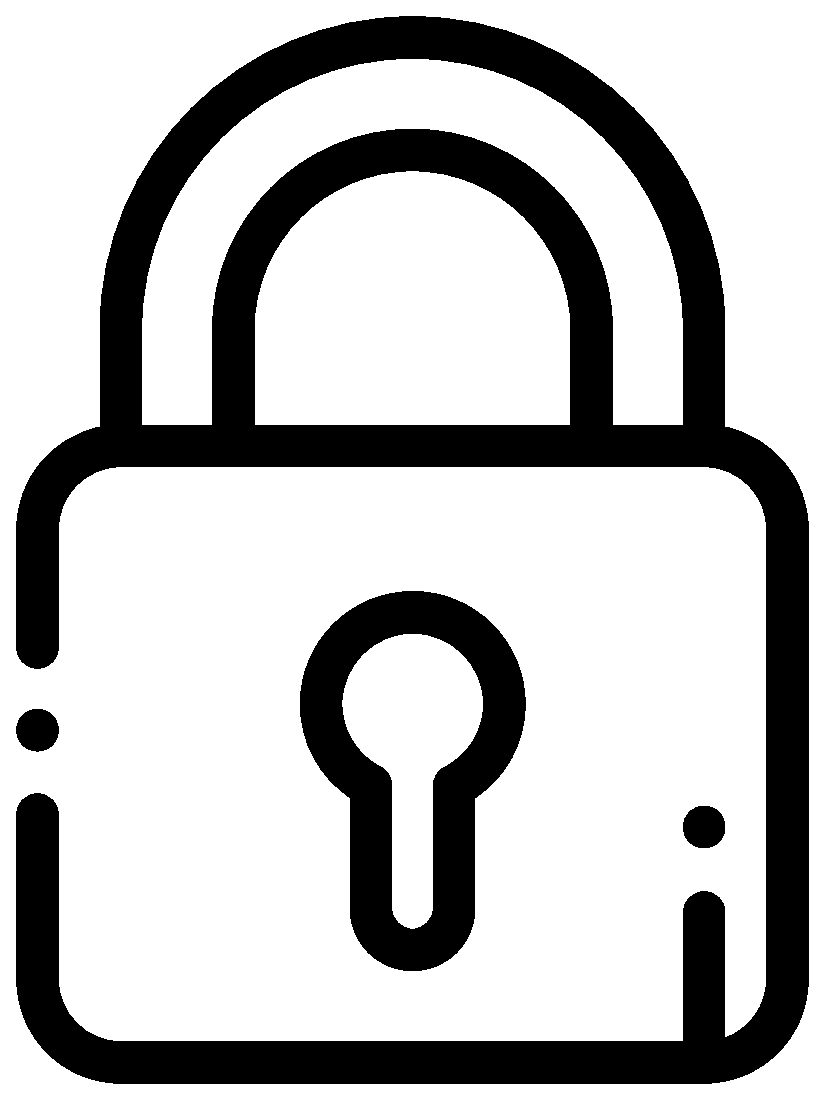
\includegraphics[width=0.5cm]{figs/icons/lock.eps}};
  \node[below=0cm of input] {$\Upsilon = Role_A $};
  \coordinate (mid) at ($(input)!.4!(user-mid)$);
  \draw (input.east) -- (mid);
  \draw[-latex] (mid) |- (user1.west) node[pos=0.75, sloped, scale=1, color=Green] {\ding{52}};
  \draw[-latex] (mid) |- (user2.west) node[pos=0.75, sloped, scale=1, color=Red] {\ding{55}};
\end{tikzpicture}
}
          \caption{Access Control}
        }
      \end{figure}
    \end{column}
    \begin{column}{0.33\linewidth}
      \begin{figure}
        \onslide<5->{%
          \resizebox{\linewidth}{!}{\begin{tikzpicture}
  \node[matrix,inner sep=0.01cm,draw=black,ellipse,dashed] (server) {%
    \node (s1) {\includegraphics[width=0.5cm]{./figs/icons/server.eps}};
    \node[below=0 of s1.south east, anchor=north west] (s2) {\includegraphics[width=0.5cm]{./figs/icons/server.eps}};
    \node[below=0 of s1.south west, anchor=north east] (s3) {\includegraphics[width=0.5cm]{./figs/icons/server.eps}};
    \\
  };

  \node[scale=0.9,left=2cm of server] (user) {\includegraphics{./figs/icons/user.eps}};
  \draw[-latex] (user) -- (server) node[midway, above, color=Red] {$q: \langle k, loc \rangle$};
\end{tikzpicture}
}
          \caption{Distributed Query Processing}
        }
      \end{figure}
    \end{column}
  \end{columns}
\end{frame}

\section{Authenticating Aggregate Queries over Set-Valued Data}

\begin{frame}[fragile]{Example of Aggregate Queries over Set-Valued Data}
  \begin{columns}
    \begin{column}{.5\linewidth}
      \setbeamercovered{transparent}
      \begin{table}
        \resizebox{\linewidth}{!}{%
          \begin{tabular}{ccl}
            \toprule
            \textbf{PID} & \textbf{ZIP} & \multicolumn{1}{c}{\textbf{Mut-Genes}}\\
            \midrule
            \onslide<1,2,3>{P1&95014&\alert<2>{A-C130R}, P-I696M} \\
            \onslide<1,3,4>{P2&20482&H-C282Y, \alert<4>{P-P12A}, \alert<3,4>{R-G1886S}} \\
            \onslide<1,2,3>{P3&95014&\alert<2>{A-C130R}, U-G71R, W-R611H} \\
            \onslide<1,3>{P4&01720&A-V2050L, H-C282Y, M-R52C, U-G71R} \\
            \onslide<1,3,4>{P5&20134&A-C130R, \alert<4>{P-P12A}, \alert<3,4>{R-G1886S}, S-E366K} \\
            \onslide<1,3>{P6&17868& C-R102G, \alert<3>{R-G1886S}} \\
            \onslide<1,3>{P7&55410&C-R102G, C-Q1334H, S-E288V} \\
            \onslide<1,3,4>{P8&20852&C-R102G, \alert<4>{P-P12A}, \alert<3,4>{R-G1886S}, K-T220M} \\
            \bottomrule
          \end{tabular}
        }
        \caption{Set-Valued Genome Dataset~\cite{pgp}}
      \end{table}
    \end{column}%
    \begin{column}{.5\linewidth}
      \begin{itemize}[<+(1)->]
        \item \textbf{Q1}: Find the most common gene in the district of Cupertino, CA (ZIP\@: 95014) \\
          \textcolor{Violet}{\emph{Answer:} \{`A-C130R'\}}
        \item \textbf{Q2}: Count the number of participants who carry the gene `R-G1886S' \\
          \textcolor{Violet}{\emph{Answer:} 4}
        \item \textbf{Q3}: Find the most frequent genes with supports $\ge$ 3 in ZIPs 20*** \\
          \textcolor{Violet}{\emph{Answer:} \{`P-P12A', `R-G1886S'\}}
      \end{itemize}
    \end{column}
  \end{columns}
\end{frame}

\begin{frame}{Problem Definition}
  \begin{itemize}[<+->]
    \item \textbf{Dataset} $\mathbb{D} = \{o_1, o_2, \dots, o_n\}$
      \begin{itemize}[<.->]
        \item $o_i = \langle A_i, X_i \rangle$.
        \item $A_i$ is a set of \textcolor{Green}{non-sensitive} attributes
        \item $X_i$ is a \textcolor{Red}{sensitive} multiset of \emph{features}
      \end{itemize}
    \item \textbf{Aggregate Query} $Q = (q, \{x_i\}, [\alpha, \beta])$
      \begin{itemize}[<.->]
        \item $q$ is an aggregate operator, i.e., \emph{max/min}, \emph{count}, \emph{sum}, \emph{top-$k$}, and \emph{frequent feature query (FFQ)}
        \item $\{x_i\}$ is the queried feature specified for \emph{count} and \emph{sum}
        \item $[\alpha, \beta]$ specifies the selection range over the \textcolor{Green}{non-sensitive} attributes
      \end{itemize}
    \item \textbf{Threat Model}
      \begin{itemize}[<.->]
        \item \alert{Integrity}: SP should prove the \emph{soundness} and \emph{completeness} of the results
        \item \alert{Confidentiality}: Clients should not infer any \emph{sensitive source data}
      \end{itemize}
  \end{itemize}
\end{frame}

\begin{frame}{Preliminaries}
  \begin{definition}<+->[Bilinear-Map (BM) Accumulator]
    Let $g$ be the group generator of a cyclic multiplicative group $\mathbb{G}$ and $s$ be a \textcolor{Red}{private value of DO}. The accumulator maps a multiset $X = \{ x_1, x_2, \dotsc, x_m \}$ to a single value in $\mathbb{G}$:
    \begin{align*}
      acc(X) = g^{P(X)} = g^{\prod_{x_i \in X}(x_i + s)}
    \end{align*}
    Without knowing $s$, one can still compute an $acc(\cdot)$ value by giving $g^s, g^{s^2}, \dotsc$
  \end{definition}
  \begin{example}<+->
    $X = \{ 1, 1, 2 \}$, $acc(X) = g^{(1+s)^2(2+s)} = g^{s^3+4 s^2+5 s+2} = g^{s^3} \cdot (g^{s^2})^4 \cdot(g^s)^5 \cdot g^2$
  \end{example}
  \begin{definition}<+->[Randomized BM Accumulator]
    BM accumulator is \alert{deterministic} for \emph{a fixed multiset}. As such, an adversary can tell in high confidence that two multisets are the same. We can randomize BM accumulator as following:
    \begin{align*}
      acc(X) = g^{P(X) \cdot r_X} = g^{r_X\prod_{x_i \in X}(x_i + s)}
    \end{align*}
    $r_X$ is a random value \textcolor{Red}{hidden from Clients} but \textcolor{Green}{disclosed to SP}
  \end{definition}
\end{frame}

\begin{frame}{Preliminaries}
  \begin{definition}[Cryptographic Hash Function]
    A cryptographic hash function $H(\cdot)$ accepts an arbitrary-length string as its input and returns a fixed-length bit string such that it is computationally infeasible to find $m_1 \neq m_2$ and $H(m_1) = H(m_2)$.
  \end{definition}
  \begin{definition}[Bilinear Pairing]
    Let $\mathbb{G}, \mathbb{G}_T$ be two cyclic multiplicative groups of order $p$.
    A pairing is a map $e: \mathbb{G} \times \mathbb{G} \to \mathbb{G}_T$, which satisfies:
    \begin{itemize}
      \item \textbf{Bilinearity}: $e(u^a,v^b) = {e(u,v)}^{ab}$, $\forall u, v \in \mathbb{G}$
      \item \textbf{Non-degeneracy}: $e(g,g) \ne 1$
      \item \textbf{Computability}: Given $u, v \in \mathbb{G}$, it is easy to compute $e(u, v)$
    \end{itemize}
  \end{definition}
\end{frame}

\begin{frame}[fragile]{PA$^2$ Authentication Framework Overview}
  \begin{figure}
    \onslide<+->{%
      \resizebox{.8\linewidth}{!}{%
        \begin{tikzpicture}
          \node[anchor=south west,inner sep=0] (A) at (0,0)
            {\includegraphics[width=\linewidth]{figs/aggregate-queries/overview.pdf}};
          \coordinate (multiset1) at (8.6,2.2);
          \coordinate (multiset2) at (11.9,3.45);
          \coordinate (aggregate1) at (9,0.1);
          \coordinate (aggregate2) at (11.7,1.55);
          \coordinate (select1) at (4.8,0.1);
          \coordinate (select2) at (7.57,3.45);
          \draw<2>[Red,ultra thick] (multiset1) rectangle (multiset2);
          \fill<2>[draw=none,fill=black,fill opacity=0.3,even odd rule]
            (A.south west) rectangle (A.north east)
            (multiset1) rectangle (multiset2);
          \draw<3>[Red,ultra thick] (aggregate1) rectangle (aggregate2);
          \fill<3>[draw=none,fill=black,fill opacity=0.3,even odd rule]
            (A.south west) rectangle (A.north east)
            (aggregate1) rectangle (aggregate2);
          \draw<4>[Red,ultra thick] (select1) rectangle (select2);
          \fill<4>[draw=none,fill=black,fill opacity=0.3,even odd rule]
            (A.south west) rectangle (A.north east)
            (select1) rectangle (select2);
        \end{tikzpicture}
      }
      \caption{Privacy-Preserving Authentication Framework for Aggregate Queries}
    }
  \end{figure}
  \begin{itemize}[<+- | alert@+>]
    \item PA$^2$ Protocols on Multiset Operations
    \item PA$^2$ Algorithms on Aggregate Queries
    \item PA$^2$ on Candidate Object Selection
  \end{itemize}
\end{frame}

\section{Authenticating Relational Queries with Fine-Grained Access Control}

\section{Authenticating {kNN} Queries in Distributed Settings}

\section{Conclusions}

\begin{frame}[standout]
  Thanks \\
  Questions?
\end{frame}

\appendix%

\begingroup
\setbeamertemplate{frametitle continuation}{}
\begin{frame}[t,allowframebreaks]{\refname}
  \bookmark[page=\thepage,startatroot]{\refname}
  \setbeamertemplate{bibliography item}[text]
  \renewcommand*{\bibfont}{\scriptsize}
  \printbibliography[heading=none]%
\end{frame}
\endgroup

\end{document}
